\section{一些技巧}
这里所指技巧具有专题性的意义,是面向解决方案的,而不是面向功能的讲解.



\subsection{内存溢出及解决方案}

\paragraph{内存溢出}所谓内存溢出,也就是计算时出现的 Out of memoery.

\begin{figure}[htbp]
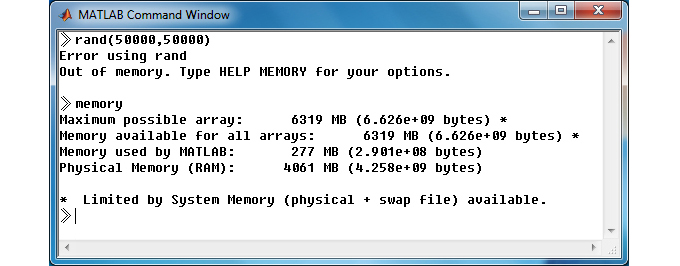
\includegraphics[width=0.6\textwidth]{diagrams/memoryout}
\caption{内存溢出和内存查看}
\end{figure}

\vspace{-0.8cm}
\begin{lstlisting}[caption = 生成随机矩阵]
  matrix = rand(2e+5,2e+5);
\end{lstlisting}

\notation{逐渐增大或减小维数,这样可以查看设备能存储最大矩阵的维数.}


\paragraph{内存溢出解决}简而言之,开源节流.
\begindot
\item 开源方法
\begin{itemize*}
\item 增加RAM.买个大点的内存条装上;
\item 以“no java”方式启动MATLAB.(这是在节MATLAB的流,开程序执行的源)
\end{itemize*}
\item 节流方法
\begin{itemize*}
\item 数据本地存储.将数据存储到本地,需要时再导入;
\item 使用已有的变量,即时删除临时变量(不再需要的变量);
\item 以函数封装.将程序中某几部分的代码封装为 function 调用, function调用只输出最后需要的数据,其间的临时变量在每次调用完function之后都会自动删除.
\end{itemize*}
\myenddot



\subsection{自定义函数帮助}
在MATLAB中可以用输入help加函数名来获得获悉使用方法及例子.我们期望对自己编写的函数也实现这样的功能,那么有两个关键点,一是参照MATLAB的内置函数注释格式写好注释(或者参照下面的示例),二是确保此函数路径已经添加.接下来就可以通过 \mcode{help myfunction} 这样的形式来查看了.

\vspace{-0.8cm}
\begin{lstlisting}[caption = 自定义帮助]
  function outputs = myfunction(inputs)
  %MYFUNCTION this function is bulabula...
  %   decrible your function here
  %   see also function1 function2

  %   Reversion: 22-Aug-2013
  %   2013/08/22  16:58:27
\end{lstlisting}



\subsection{图像导出}
除了一般的截图方法,有这样几种方法.

\begindot
\item \mcode{print('-dpdf',pdf_name);},生成图像为pdf格式.
\item 直接设置导出, File - Export Setup - Export, 通过 Rendering - Resolution 可以设置图像质量.
\item \mcode{saveas(gcf, 'output', 'jpg')}, 导出当前figure为名为output的jpg格式图像.
\myenddot



\subsection{公式打印}
MATLAB支持\LaTeX 的公式输出,在两个地方可能用到公式输出.

\begindot
\item 图片上的公式
\item 代码发布注释中的公式
\myenddot

\vspace{-0.8cm}
\begin{lstlisting}[caption = 图像中的公式输出]
  y = title('$$y = \sqrt{x}$$');		% 标题
  set(y,'interpreter','latex');			% 用LaTeX翻译标题
\end{lstlisting}



\subsection{重复向量以构造矩阵}
首先解释一下什么是向量重复构造矩阵,比如有一个向量 \mcode{[1 2 3]},现在我打算将它构造成 \mcode{[1 2 3; 1 2 3; 1 2 3]},这就是此小节要解决的内容.

\vspace{-0.8cm}
\begin{lstlisting}[caption = 重复向量以构造矩阵]
  %% repmat 函数方法
  clear
  x = 1:1:20000; N = 30000;
  tic
  X = repmat(x, N, 1);
  toc

  %% 矩阵乘法方法
  clear
  x = 1:1:20000; N = 30000;
  tic
  Y = ones(N,1)*x;
  toc
  
  %% 下标方法
  clear
  x = 1:1:20000; N = 30000;
  tic
  Z = x(ones(N, 1), :);
  toc
\end{lstlisting}

\vspace{-0.8cm}
\begin{lstlisting}
  Elapsed time is 25.953179 seconds.
  Elapsed time is 217.866385 seconds.
  Elapsed time is 13.400210 seconds.
\end{lstlisting}

实际上, \mcode{repmat} 用到了第三种,在其源码中可以看的到,但它更加通用.如果是数值,首推第三者.
 \mcode{repmat} 的源码可以通过 \mcode{which repmat} 查看其位置. 另外需要提及,测试时每段前面当加 \mcode{clear},这是要消除由于内存的原因影响后面程序的执行效率.\par

还有一种方式,这种方式可以列重复挨着:

\vspace{-0.4cm}
\begin{lstlisting}
  >> blkproc([1 2 3 4 5], [1 1], @(x)repmat(x, 3, 2))

  ans =

  1     1     2     2     3     3     4     4     5     5
  1     1     2     2     3     3     4     4     5     5
  1     1     2     2     3     3     4     4     5     5 
\end{lstlisting}

\notation{可以考虑用上面的某种方法用向量重复来构造三维的矩阵.}